\documentclass[conference,harvard,brazil,english]{sbatex}
\usepackage[utf8]{inputenc}
\usepackage[T1]{fontenc}
\usepackage{ae}
\usepackage{graphicx}
\usepackage{epsfig}
\usepackage{url}
\usepackage{subcaption}
\usepackage{graphics}
\makeatletter
\def\verbatim@font{\normalfont\ttfamily\footnotesize}
\makeatother
\usepackage{amsmath}
\usepackage{float}
\usepackage{listings}
\usepackage{color}
%\usepackage{xcolor}
\definecolor{lightgray}{rgb}{.9,.9,.9}
\definecolor{darkgray}{rgb}{.4,.4,.4}
\definecolor{purple}{rgb}{0.65, 0.12, 0.82}


\lstdefinelanguage{JavaScript}{
  keywords={typeof, new, true, false, catch, function, return, null, catch, switch, var, if, in, while, do, else, case, break},
  keywordstyle=\color{blue}\bfseries,
  ndkeywords={class, export, boolean, throw, implements, import, this},
  ndkeywordstyle=\color{darkgray}\bfseries,
  identifierstyle=\color{black},
  sensitive=false,
  comment=[l]{//},
  morecomment=[s]{/*}{*/},
  commentstyle=\color{purple}\ttfamily,
  stringstyle=\color{red}\ttfamily,
  morestring=[b]',
  morestring=[b]"
}
% \lstset { %
% 	language = JavaScript,
%     backgroundcolor=\color{black!5}, % set backgroundcolor
%     basicstyle=\footnotesize,% basic font setting
%     breakatwhitespace=true
%    breaklines=true,
% }
\lstset{
   language=JavaScript,
   backgroundcolor=\color{lightgray},
   extendedchars=true,
   basicstyle=\footnotesize\ttfamily,
   showstringspaces=false,
   showspaces=false,
%   numbers=left,
%   numberstyle=\footnotesize,
%   numbersep=9pt,
   tabsize=2,
   breaklines=true,
   showtabs=false,
   captionpos=b
}

% --------------------------------------------------


%\usepackage[portuguese]{babel}
%\selectlanguage{portuguese}
\begin{document}

% CABEÇALHO

\title{Morfologia matemática}

%%%%%%%%%%%%%%%%%%%%%%%%%%%%%%%%%%%%%%%%%%%%%%%%%%%%%%%%%%%%%
%
% O processo de revisao do CBA 2014 sera DOUBLE BLIND, portanto NAO inclua
% autores na versão que será submetida para revisão
%
%%%%%%%%%%%%%%%%%%%%%%%%%%%%%%%%%%%%%%%%%%%%%%%%%%%%%%%%%%%%%

\author{Gabriel Teixeira Vantuil}{gabrieltvantuil@gmail.com}
\address{Natal, RN, Brasil}


\twocolumn[

\maketitle

\selectlanguage{english}
\begin{abstract}
The goal of this job is the development of a web page that can run mathematical morphology algorithms with a user interface, in order to help teaching digital image processing. 
  \end{abstract}

\keywords{Morphology, erode, dilate, computer-vision.}

\selectlanguage{brazil}
\begin{abstract}
	O objetivo desse trabalho é desenvolver uma página web que execute o processo de morfologia matemática com uma interface de modo que auxilie o ensino de processamento digital de imagens. 
\end{abstract}

\keywords{Morfologia, erosão, dilatação, visão computacional}
]

% CONTRIBUIÇÃO

\selectlanguage{brazil}

\section{Introdução }
A morfologia é em sua essência, o estudo da forma. Por exemplo, morfologia vegetal é o estudo da estrutura dos vegetais.

A morfologia matemática utiliza um elemento estruturante, definido pelo usuário, para realizar as operações na geometria tratada. No contexto de processamento de imagens, a geometria a ser tratada é uma imagem, e o elemento estruturante pode ser de diversos formas, a depender da aplicação. 

Para facilitar as operações o elemento estruturante é formado por matrizes de poucos elementos e geralmente quadradas. São compostos de pixels de fundo e pixels ativos, ou seja, pixels que irão interagir com a geometria (ativos) ou não (fundo). O pixel central do elemento estruturante é a referência ao redor da qual serão executadas as operações. 
Alguns dos elementos estruturantes mais comuns são, onde "\(\bullet\)" representa pixels ativos e "." representa pixels fundo:
\[
\begin{bmatrix}
    . & . & \bullet & . & . \\
    . & \bullet & \bullet & \bullet & . \\
    \bullet & \bullet & \bullet & \bullet & \bullet \\
    . & \bullet & \bullet & \bullet & . \\
    . & . & \bullet & . & . \\
\end{bmatrix},
\]
\[
\begin{bmatrix}
    . & . & . \\
    \bullet & \bullet & \bullet \\
    . & . & . \\
\end{bmatrix}, 
\begin{bmatrix}
    . & \bullet & . \\
    . & \bullet & . \\
    . & \bullet & . \\
\end{bmatrix}, 
\begin{bmatrix}
    . & \bullet & . \\
    \bullet & \bullet & \bullet \\
    . & \bullet & . \\
\end{bmatrix}, 
\begin{bmatrix}
    \bullet & \bullet & \bullet \\
    \bullet & \bullet & \bullet \\
    \bullet & \bullet & \bullet \\
\end{bmatrix}
\]

As operações morfológicas são uma parte importante do processamento digital de imagens, são comumente utilizadas nos primeiros processos de tratamento de imagens, pois são capazes de eliminar ruídos provenientes de uma má qualidade de captura da imagem. Se trata de um processo barato computacionalmente (são simples cálculos matemáticos, portanto pode ser realizado por hardware de forma mais eficiente).

\section{Fundamentação teórica}
\subsection{Operações fundamentais}

As duas operações fundamentais da morfologia matemática são erosão e dilatação.

Erosão, como o nome sugere, faz com que os pixels de fundo se sobresaiam em relação aos pixels ativos. 

Para tal, no contexto de imagens binárias é realizada uma comparação entre os pixels do elemento estruturante e a geometria, de forma que para cada pixel da imagem, é verificado se todos os pixels ativos no elemento estruturante estão ativos na geometria. Ou seja, se for realizada a erosão em uma geometria igual ao elemento estruturante, apenas o pixel central irá se manter, pois é necessário que todos os pixels do elemento sejam iguais ao da geometria, caso contrário, o pixel analisado será removido.

Por exemplo, se for aplicado o seguinte elemento estruturante:
\\
\[\begin{bmatrix}
    \bullet & \bullet & \bullet \\
    \bullet & \bullet & \bullet \\
    \bullet & \bullet & \bullet \\
\end{bmatrix}\]
\\ na Figura \ref{operacoes_in} a geometria resultante é \ref{operacoes_e} para a operação de erosão.
\begin{figure}[htp]
\centering
	\begin{subfigure}{0.5\textwidth}
	    \centering
		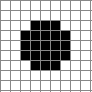
\includegraphics[width=3cm]{pdi_in.PNG}
    	\caption{entrada}
		\label{operacoes_in}
  	\end{subfigure}
	\begin{subfigure}{0.5\textwidth}
	    \centering
      	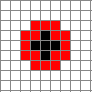
\includegraphics[width=3cm]{pdi_erode.PNG}
      	\caption{saída erosão}
		\label{operacoes_e}
    \end{subfigure}
	\begin{subfigure}{0.5\textwidth}
	    \centering
      	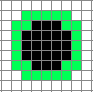
\includegraphics[width=3cm]{pdi_dilate.PNG}
      	\caption{saída dilatação}
		\label{operacoes_d}
    \end{subfigure}
\caption{Exemplos de operações morfológicas (erode e dilate) executadas na página web desenvolvida.}
\label{operacoes}
\end{figure}

A operação de dilatação funciona de forma semelhante, porém quando um elemento estruturante é aplicado a um pixel ativo, os pixels vizinhos, seguindo o elemento estruturante definido, serão marcados como ativos. Ou seja, para uma geometria composta apenas de um pixel, o resultado da dilatação será igual ao elemento estruturante, pois a operação será realizada apenas sobre um pixel.

A Figura \ref{operacoes_d}  demonstra a saída para a operação de dilatação.
\subsection{Operações derivadas}
As operações de erosão e dilatação podem corrigir erros em imagens, porém ambas alteram o tamanho da imagem a ser corrigida, sendo diminuindo como a erosão, ou aumentando como a dilatação. Esse problema pode ser resolvido com uma técnica simples.

Duas outras operações de morfologia matemática podem ser obtidas à partir das operações básicas. Essas operações são chamadas de abertura e fechamento. Para ambas operações o mesmo elemento estruturante deve ser aplicado na erosão e dilatação, caso contrário, o resultado pode não ser o esperado, pois podem aparecer falhas de geometria.

A operação de abertura é a realização de uma erosão, seguida de uma dilatação. É muito útil para remover ruido pois no geral, não altera o tamanho da imagem e remove pixels ativos que deveriam ser fundo. Uma demonstração dessa operação pode ser vista na figura \ref{operacao_abertura}, onde o seguinte elemento estruturante foi aplicado: 
\[\begin{bmatrix}
    \bullet & \bullet & \bullet \\
    \bullet & \bullet & \bullet \\
    \bullet & \bullet & \bullet \\
\end{bmatrix}\]

\begin{figure}[htp]
\centering
	\begin{subfigure}{0.5\textwidth}
	    \centering
		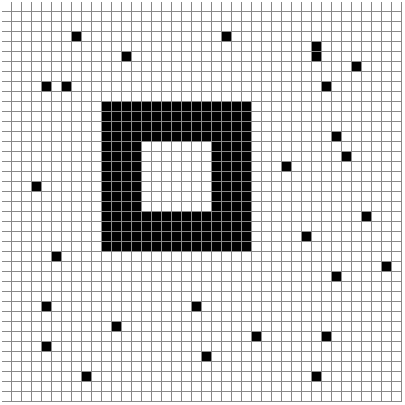
\includegraphics[width=5cm]{Abertura_original.PNG}
    	\caption{entrada}
  	\end{subfigure}
	\begin{subfigure}{0.5\textwidth}
	    \centering
      	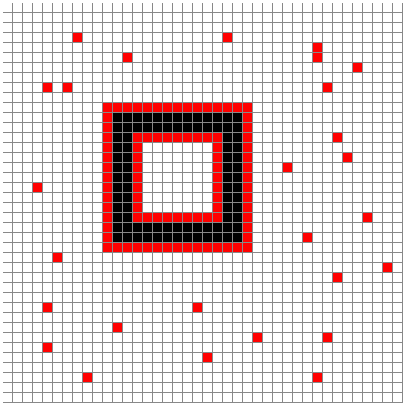
\includegraphics[width=5cm]{Abertura_erode.PNG}
      	\caption{Resultado erosão}
    \end{subfigure}
	\begin{subfigure}{0.5\textwidth}
	    \centering
      	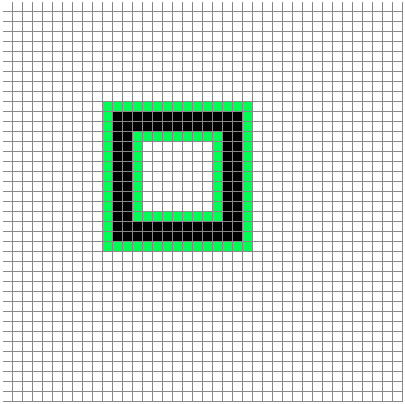
\includegraphics[width=5cm]{Abertura_dilate.PNG}
      	\caption{Resultado dilatação}
    \end{subfigure}
\caption{Exemplos de operação morfológica abertura executadas na página web desenvolvida.}
\label{operacao_abertura}
\end{figure}

Já a operação de fechamento, é a realização de uma dilatação, seguida de uma erosão, é portanto o oposto da abertura. Assim como a abertura, pode ser usada para remover ruido e também não altera o tamanho da imagem. O fechamento, remove pixels de fundo inseridos na geometria desejada. Uma demonstração dessa operação pode ser vista na figura \ref{operacao_fechamento}.

\begin{figure}[htp]
\centering
	\begin{subfigure}{0.5\textwidth}
	    \centering
		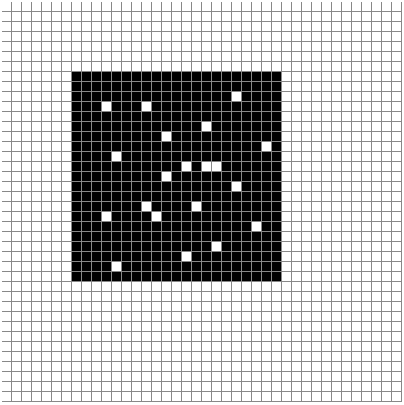
\includegraphics[width=6cm]{Fechamento_original.PNG}
    	\caption{entrada}
  	\end{subfigure}
	\begin{subfigure}{0.5\textwidth}
	    \centering
      	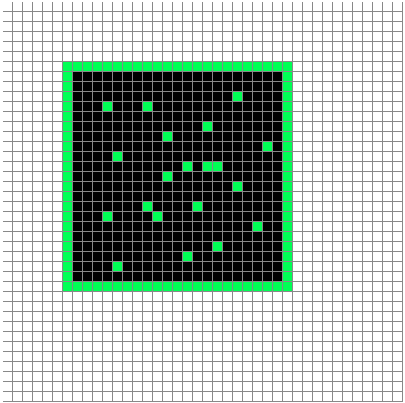
\includegraphics[width=6cm]{Fechamento_dilate.PNG}
      	\caption{Resultado dilatação}
    \end{subfigure}
	\begin{subfigure}{0.5\textwidth}
	    \centering
      	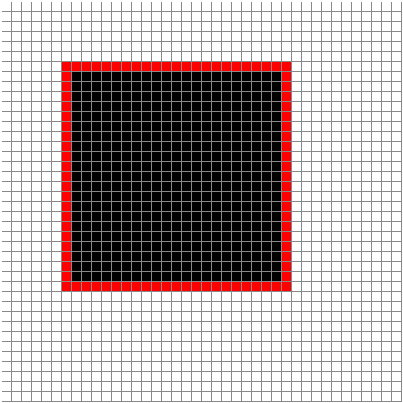
\includegraphics[width=6cm]{Fechamento_erode.PNG}
      	\caption{Resultado erosão}
    \end{subfigure}
\caption{Exemplos de operação morfológica abertura executadas na página web desenvolvida.}
\label{operacao_fechamento}
\end{figure}


\section{Desenvolvimento}
O desenvolvimento da página web foi feito utilizando HTML, CSS e Javascript, o código HTML é a parte responsável por descrever o formato básico da página, bem como a posição de cada elemento da página. O CSS descreve comportamentos estéticos da página, como cores de cada elemento organização interna dos elementos, como margens, posição de outros elementos que estão dentro de um elemento maior. Javascript executa os algoritmos referentes às operações morfológicas. Na figura \ref{pagina} podemos ver uma demonstração da pagina.

\begin{figure}[ht]
\centering
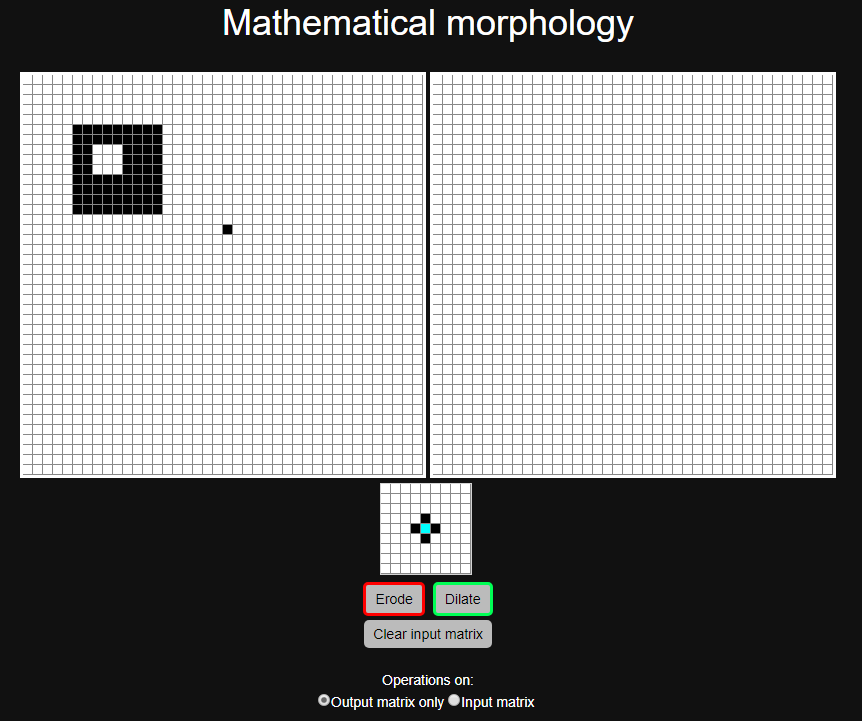
\includegraphics[width=7cm]{body.png}
\caption{Demonstração da página}
\label{pagina}
\end{figure}

\subsection{Javascript}
Javascript é uma linguagem de programação baseada em java, que por sua vez é baseada em C, é em grande parte orientada a objetos. Por ter grande parte de sua sintaxe similar a C++, foi uma boa escolha para tratar do backend da página. Possui fácil integração com o HTML, de modo que basta definir uma "id" no HTML e declarar uma variável em Javascript para fazer a conexão entre as duas linguagens, como por exemplo: 
\textit{var div = document.getElementById("id\_div");}, nesse exemplo, a variável \textit{div} está diretamente relacionada ao elemento que tiver a identificação "id\_div" no código HTML. Outra facilidade dessa linguagem é a orientação a eventos, ou seja, não é necessário criar um codigo para verificar se algo está acontecendo. Basta definir que quando algo acontecer, uma função seja chamada.
Por exemplo: \textit{div.onclick =  function()\{ funcao(A,B);\};}, ou seja, quando \textit{div} for clicada, uma função será disparada. Sendo que não é necessário deixar um laço de repetição para lidar com esse evento, pois já é nativo da linguagem, o trecho de código necessita ser escrito apenas uma vez em algum lugar que quando for lido, a ligação entre o elemento e a função será estabelecida.

\subsection{Canvas}
Canvas, de acordo com [2] é um elemento web desenvolvido com o propósito de criar animações/ilustrações/desenhos no geral, a partir de comandos em Javascript. A escolha do canvas foi feita pois através de poucas funções é possível desenhar no elemento.
Alguns dos métodos utilizados para manipulação do elemento canvas são:
\begin{itemize}
\item getContext("2d"): define a renderização do canvas como bidimensional.
\item fillStyle: define a cor que será preenchida na geometria a ser inserida (caminho). É necessário alguma outra função para efetivamente desenhar a figura.
\item beginPath(): Inicia um caminho de desenho. Função necessária antes de alguma função de desenho, pois caso contrário, não é possível mudar a cor da figura a desenhada. Ou até mesmo, se não for incluída essa função, uma figura anteriormente desenhada pode ter sua cor alterada. 
\item fillRect(Px0,Py0,sizeX,sizeY): Adiciona um retângulo iniciando em (Px0,Py0) e com o tamanho (sizeX,sizeY), ao caminho criado.
\item stroke(): Desenha os caminhos anteriormente definidos.
\item getImageData(Px0,Py0,sizeX,sizeY).data: o método \textit{getImageData()} retorna uma cópia da região selecionada. A propriedade \textit{.data} retorna a cor dessa região. Nesse algoritmo, o sizeX e sizeY são iguais a 1.

\end{itemize}


\subsection{Código}
O desenvolvimento do código se baseia em \textit{canvas} e javascript.
A manipulação das imagens foi feita utilizando apenas dois métodos principais de desenho no canvas, um para verificação de cor do pixel, outro para desenhar um retângulo. Utilizando esses métodos, foram desenvolvidas funções para definir o que ao longo dessa explicação, chamarei de pixels virtuais, que não são realmente pixels, pois cada um é composto de um conjunto de pixels reais, ou seja, a menor unidade de um monitor. Esses pixels virtuais foram definidos visando uma interface mais amigável e intuitiva.

As funções de consulta e definição dos pixels virtuais criadas são:
\begin{lstlisting}
function setPixel(c, i, j, cor){
  var ctx = c.getContext("2d"); 
  ctx.fillStyle=cor;
  ctx.beginPath();
  ctx.fillRect(i*(px_size+1),j*(px_size+1),px_size,px_size);
  ctx.stroke();
}
function getPixel(c, i, j) {
  var ctx = c.getContext("2d");
  var pix = ctx.getImageData(i*(px_size+1)+ px_size/2,j*(px_size+1)+ px_size/2, 1, 1).data;  
  var px= "#" + (pix[0]/16).toString(16)[0] + (pix[1]/16).toString(16)[0]+(pix[2]/16).toString(16)[0];
    return px;
}
\end{lstlisting}
A função setPixel() desenha um quadrado (pixel virtual) de lado \textit{px\_size}(pixels reais)  no canvas \textit{c}, na posição \textit{i,j}: posição definida respeitando o tamanho de cada pixel virtual (constante \textit{px\_size}) e somando 1 (referente ao espaço entre os pixels virtuais).
Ou seja, essa função desenha os quadrados apenas em uma matriz de pixels virtuais, de forma a simular um arquivo real.

A função getPixel() resgata as informações de cor do pixel virtual \textit{i,j} do canvas \textit{c}. Alguns tratamentos foram necessários para selecionar a cor central do pixel virtual, pois embora todo o pixel seja da mesma cor, as bordas são de cores diferentes, e função do canvas que retorna a cor de um pixel, utiliza coordenadas reais do canvas (em pixels reais).

A forma de entrada da imagem a ser tratada, bem como o canvas que define o elemento estruturante, foi a aquisição de dados do mouse, essa aquisição é feita pelo seguinte trecho de código:

\begin{lstlisting}
var canvas = document.getElementById("input");
canvas.onmousedown  = function(){ pressed(this,event);};
canvas.onmouseup    = function(){ isclicked=0;};
canvas.onmouseout   = function(){ isclicked=0;};
canvas.onmousemove  = function(){ setPixel_input(this,event);};

var mask = document.getElementById("mask");
mask.onmousedown  = function(){ pressed(this,event);};
mask.onmouseup    = function(){ isclicked=0;};
mask.onmouseout   = function(){ isclicked=0;};
mask.onmousemove  = function(){ setPixel_input(this,event);};
\end{lstlisting}
Onde a variável \textit{canvas} a matriz de entrada e \textit{mask} é o elemento estruturante.
E o evento: 
\begin{itemize}
\item onmousedown: chama a função \textit{pressed()} quando algum ponto do canvas correspondente for pressionado;
\item onmouseup: zera a variável \textit{isclicked} quando o botão do mouse for solto;
\item onmouseout: zera a variável \textit{isclicked} quando o mouse sair da área do canvas;
\item onmousemove: chama a função \textit{setPixel\_input()} toda vez que o mouse se deslocar no canvas.
\end{itemize}

Esses eventos são a base para a entrada de dados no sistema. A variável \textit{isclicked} foi implementada, para que, juntamente com a função \textit{pressed()}, facilitar a entrada de uma quantidade maior de dados nas matrizes. Pois caso contrário, seria necessário clicar em cada pixel individualmente. Ao invés disso, quando o mouse é pressionado em um pixel, a posição desse pixel é registrada e sua cor é alternada, caso o mouse se mova sem que o botão seja solto, até que o ponteiro atinja outro pixel, nenhuma ação é realizada. Ao mover o mouse pressionado sobre um pixel, sua cor é alterada.Ao soltar o botão do mouse ou sair da área desenhável, nenhum pixel trocará de cor enquanto o botão não for pressionado novamente, ou seja, a função \textit{setPixel\_input()} que é a responsável por alternar a cor do pixel quando o mouse está em movimento, não realiza a troca de cor caso a variável \textit{isclicked} tenha valor zero. 

Essa implementação das funções \textit{setPixel\_input()} e \textit{pressed()} pode ser verificada no seguinte trecho de código:




\begin{lstlisting}
function pressed(c,event){
 if(isclicked==0){
  isclicked=1; 
  X0 = Math.floor(event.offsetX/(px_size+1)); //centro do pixel inicialmente clicado
  Y0 = Math.floor(event.offsetY/(px_size+1)); 
  setPixel_mouse(c,event);
 }
}

function setPixel_input(c,e){
 if(isclicked==1){
  var ctx = c.getContext("2d");
  var X = Math.floor(e.offsetX/(px_size+1));//centro do pixel atual
  var Y = Math.floor(e.offsetY/(px_size+1));

  if(X0 != X || Y0 != Y){
   X0 = Math.floor(e.offsetX/(px_size+1)); //centro do pixel inicialmente clicado
   Y0 = Math.floor(e.offsetY/(px_size+1));
   var px =getPixel(c, X0, Y0);
   if(px=="#fff")         //branco
    setPixel(c,X,Y,"#000");
   if(px=="#000")              //preto
    setPixel(c,X,Y,"#fff");
  }
 }
}

\end{lstlisting}

A função que realiza a morfologia em si é:

\begin{lstlisting}
function morph2(erode){
    
 quadricular(morph_output);
 var manter = document.getElementById("manter_in").checked;
 for(var i=0;i<morph_input.width/(px_size+1);i++)
 for(var j=0;j<morph_input.height/(px_size+1);j++){
  if(!erode){
   if(getPixel(morph_input,i,j) == "#000"){
    for(var im=-Math.floor(mask_size/2); im<=Math.floor(mask_size/2); im++)
    for(var jm=-Math.floor(mask_size/2); jm<=Math.floor(mask_size/2); jm++){
     if(getPixel(mask,Math.floor(mask_size/2)+im,Math.floor(mask_size/2)+jm) == "#000"){
      if(getPixel(morph_input,i+im,j+jm) == "#fff")
       setPixel(morph_output,i+im,j+jm,dilate_color);
     }
     setPixel(morph_output,i,j,"#000");
  }}}//dilate
  else{
   if(getPixel(morph_input,i,j) == "#000"){
    setPixel(morph_output,i,j,"#000");
     for(var im=-Math.floor(mask_size/2); im<=Math.floor(mask_size/2); im++)
     for(var jm=-Math.floor(mask_size/2); jm<=Math.floor(mask_size/2); jm++)
      if(getPixel(mask,Math.floor(mask_size/2)+im,Math.floor(mask_size/2)+jm)=="#000")
       if(getPixel(morph_input,i+im,j+jm) != "#000"){
        setPixel(morph_output,i,j,erode_color);
        break;
 }}}}
 for(var i=0;i<morph_input.width/(px_size+1);i++)
 for(var j=0;j<morph_input.height/(px_size+1);j++){
  if(!manter){
   if(getPixel(morph_output,i,j) == "#000" || getPixel(morph_output,i,j) == "#fff")
    setPixel(morph_input,i,j,getPixel(morph_output,i,j));
  else if(getPixel(morph_output,i,j) == erode_color)
   setPixel(morph_input,i,j,"#fff");
  else if(getPixel(morph_output,i,j) == dilate_color)
   setPixel(morph_input,i,j,"#000");
}}}

\end{lstlisting}


\subsection{Formas de Operação}
Há duas formas de utilização da aplicação web:
\begin{itemize}
\item Operações na matriz de saída
Quando essa opção está selecionada, as operações morfológicas serão realizadas apenas na matriz de saída, preservando assim, a figura desenhada na matriz de entrada. Essa abordagem é importante pois é possível ver a entrada e saída de forma clara, bem como é possível alterar a entrada e realizar novamente a operação. Como pode ser visto na fig. \ref{op_saida}

\item Operações na matriz de entrada
Quando essa opção está selecionada, as operações morfológicas serão realizadas na matriz de saída e copiadas para a matriz de entrada, sobrescrevendo a entrada anterior. Utilizando essa opção, podem ser implementados várias combinações de operações morfológicas, inclusive, as operações de abertura e fechamento. Assim como na anterior, nessa opção a matriz de saída registra o resultado da operação realizada. Na  figura \ref{op_entrada}, uma demonstração dessa opção.
\end{itemize}

\begin{figure}[htp]
	\centering
	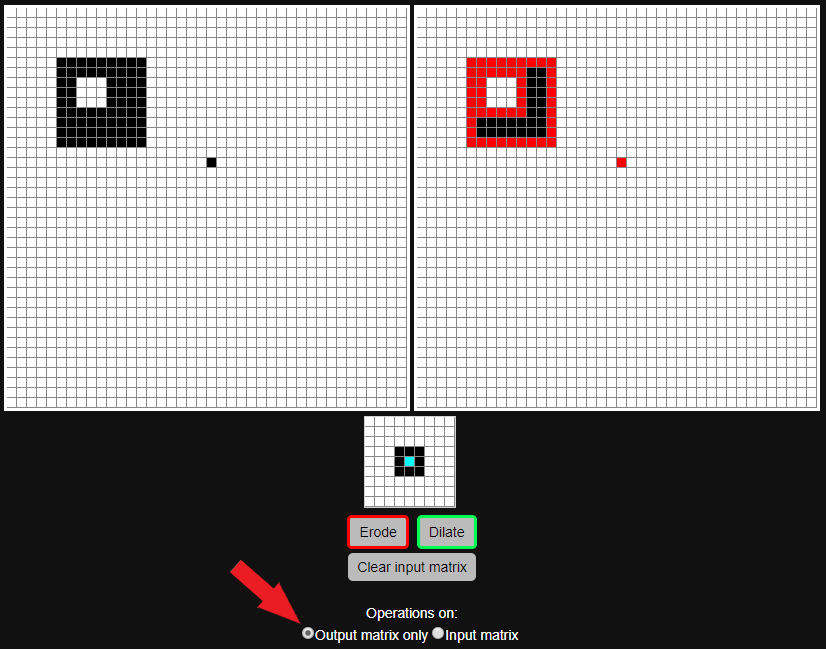
\includegraphics[width=7cm]{op_saida.png}
	\caption{Exemplo de operação apenas na matriz de saída}
	\label{op_saida}
\end{figure}

\begin{figure}[htp]
	\centering
	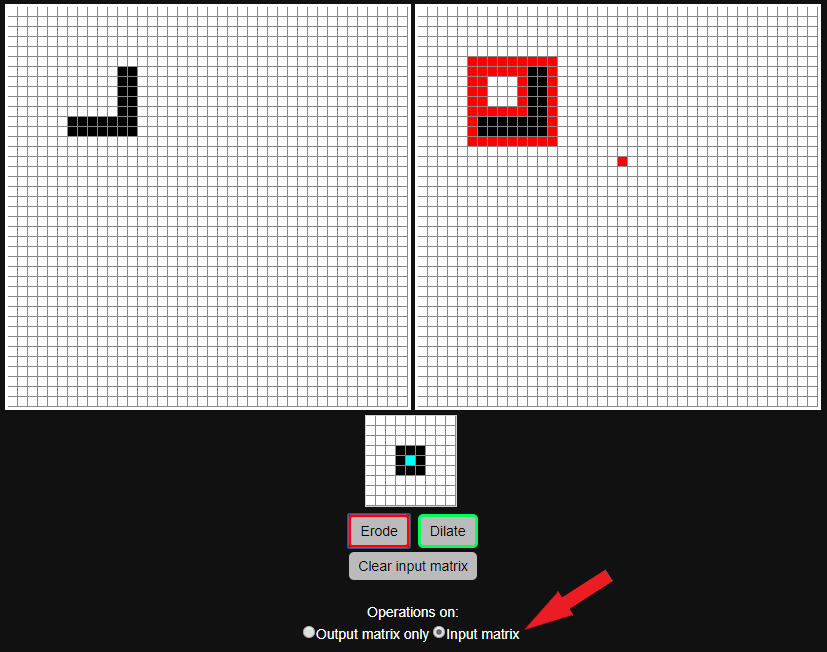
\includegraphics[width=7cm]{op_entrada.png}
	\caption{Exemplo de operação na matriz de entrada}
	\label{op_entrada}
\end{figure}


\begin{lstlisting}

\end{lstlisting}

\pagebreak
\begin{thebibliography}{99}

\bibitem{c3} Wikipedia. Available: \url{https://pt.wikipedia.org/wiki/Morfologia_matem%C3%A1tica} [Accessed: 25 - may - 2018]

\bibitem{canvas_ref} Mozilla Canvas. Available: \url{https://developer.mozilla.org/pt-BR/docs/Web/Guide/HTML/Canvas\_tutorial} [Accessed: 30 - may - 2018]

\bibitem{canvas_ref2} Mozilla Canvas. Available: \url{https://developer.mozilla.org/pt-BR/docs/Web/API/HTMLCanvasElement/getContext} [Accessed: 30 - may - 2018]

\bibitem{canvas_ref3} w3schools \url{https://www.w3schools.com/tags/canvas_getimagedata.asp} [Accessed: 30 - may - 2018]

\bibitem{minicurso} Minicurso PUC. Available: \url{https://www.ppgia.pucpr.br/~facon/Books/2011WVCMinicurso2Morfo.pdf} [Accessed: 3 - Jun - 2018]

\end{thebibliography}


\end{document}
